%!TEX root = ../../main.tex

\chapter{Vorwort}
\label{sec:chapAllgemein} 
\textbf{Login}\\
Wird die Startseite aufgerufen, kann sich der Benutzer dort anmelden. Um den Anmeldungsprozess zu starten, muss der Nutzer die Link \glqq log-in\grqq\: anklicken. 
\textcolor{magenta}{hier bild a-priori landingpage}
Dadurch wird er zur Unterseite weitergeleitet in der die Anmeldeinformationen eingetragen werden können. Zum Login werden sowohl der Benutzername als auch das Passwort benötigt. Beides wird bei der initialen Erstellung des Benutzers durch den Verwaltungsangestellten an den Benutzer versendet. Wurden diese Informationen eingetragen, kann durch einen Klick auf die Schaltfläche \glqq Login\grqq\: abgeschlossen werden.
Dies führt den Benutzer dann auf die Kursübersicht.

\begin{figure}[h]
\centering
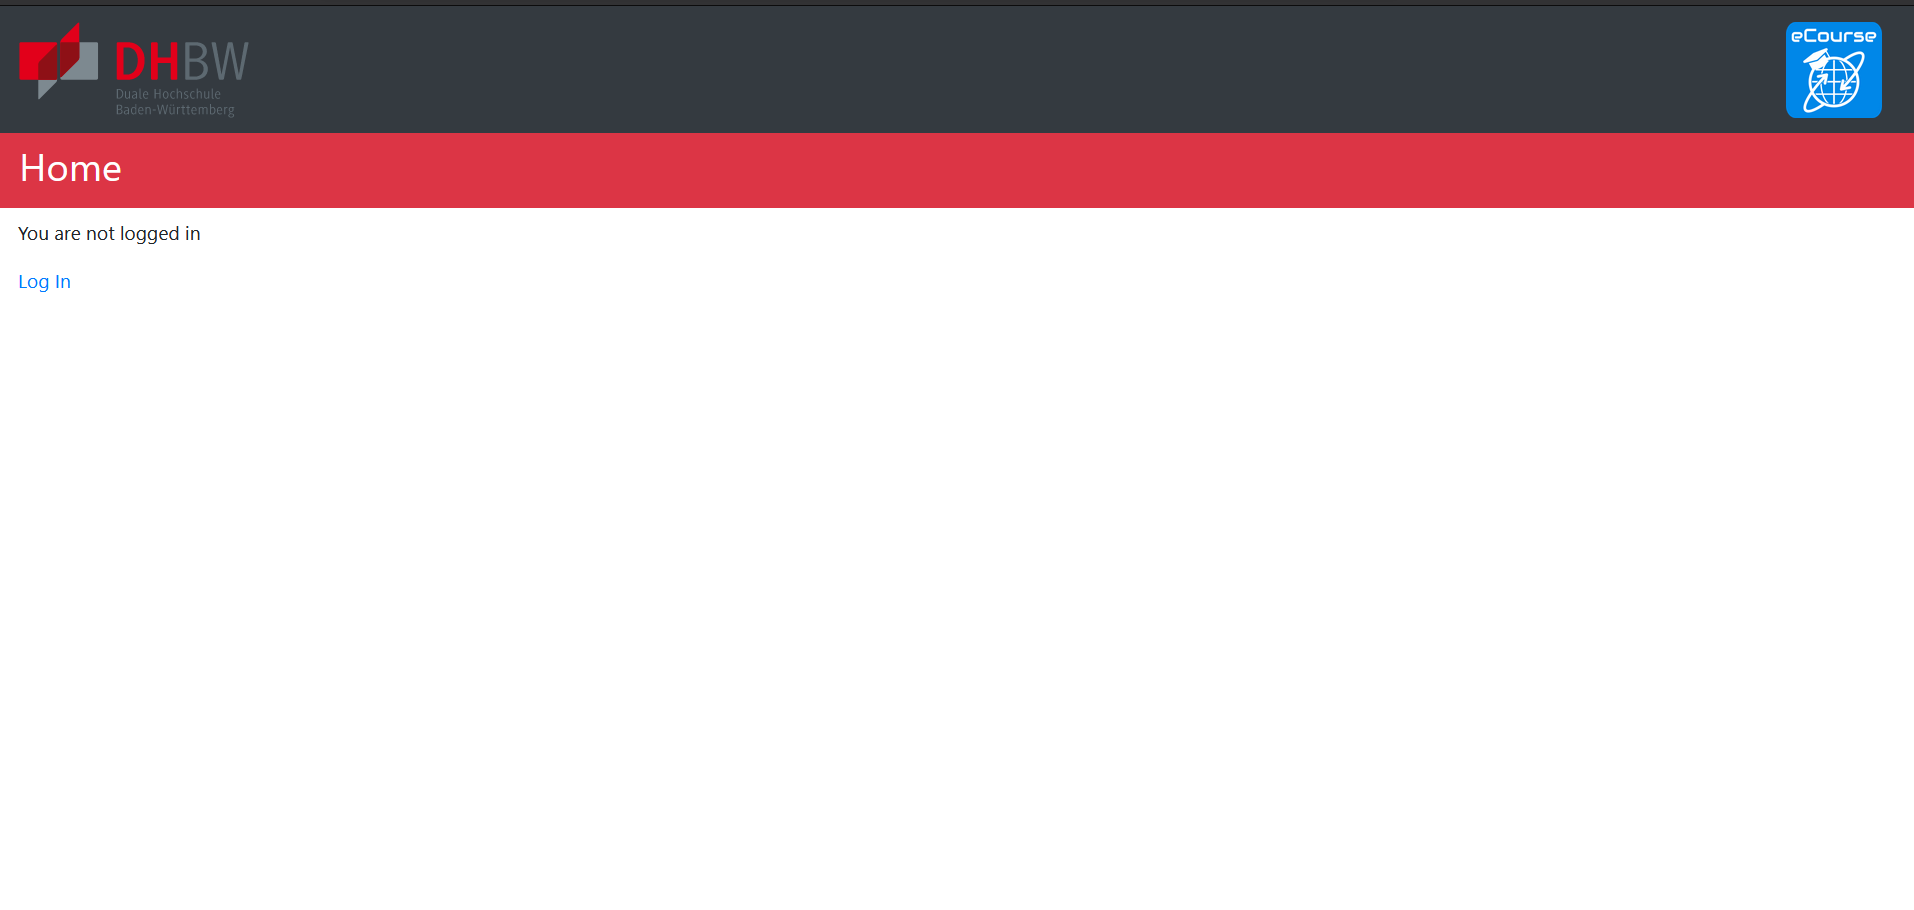
\includegraphics[height=.5\textwidth]{landing_page.png}
\caption{Startseite der Anwendung eCourse}
\label{fib:start}
\end{figure}


\begin{figure}[h]
\centering
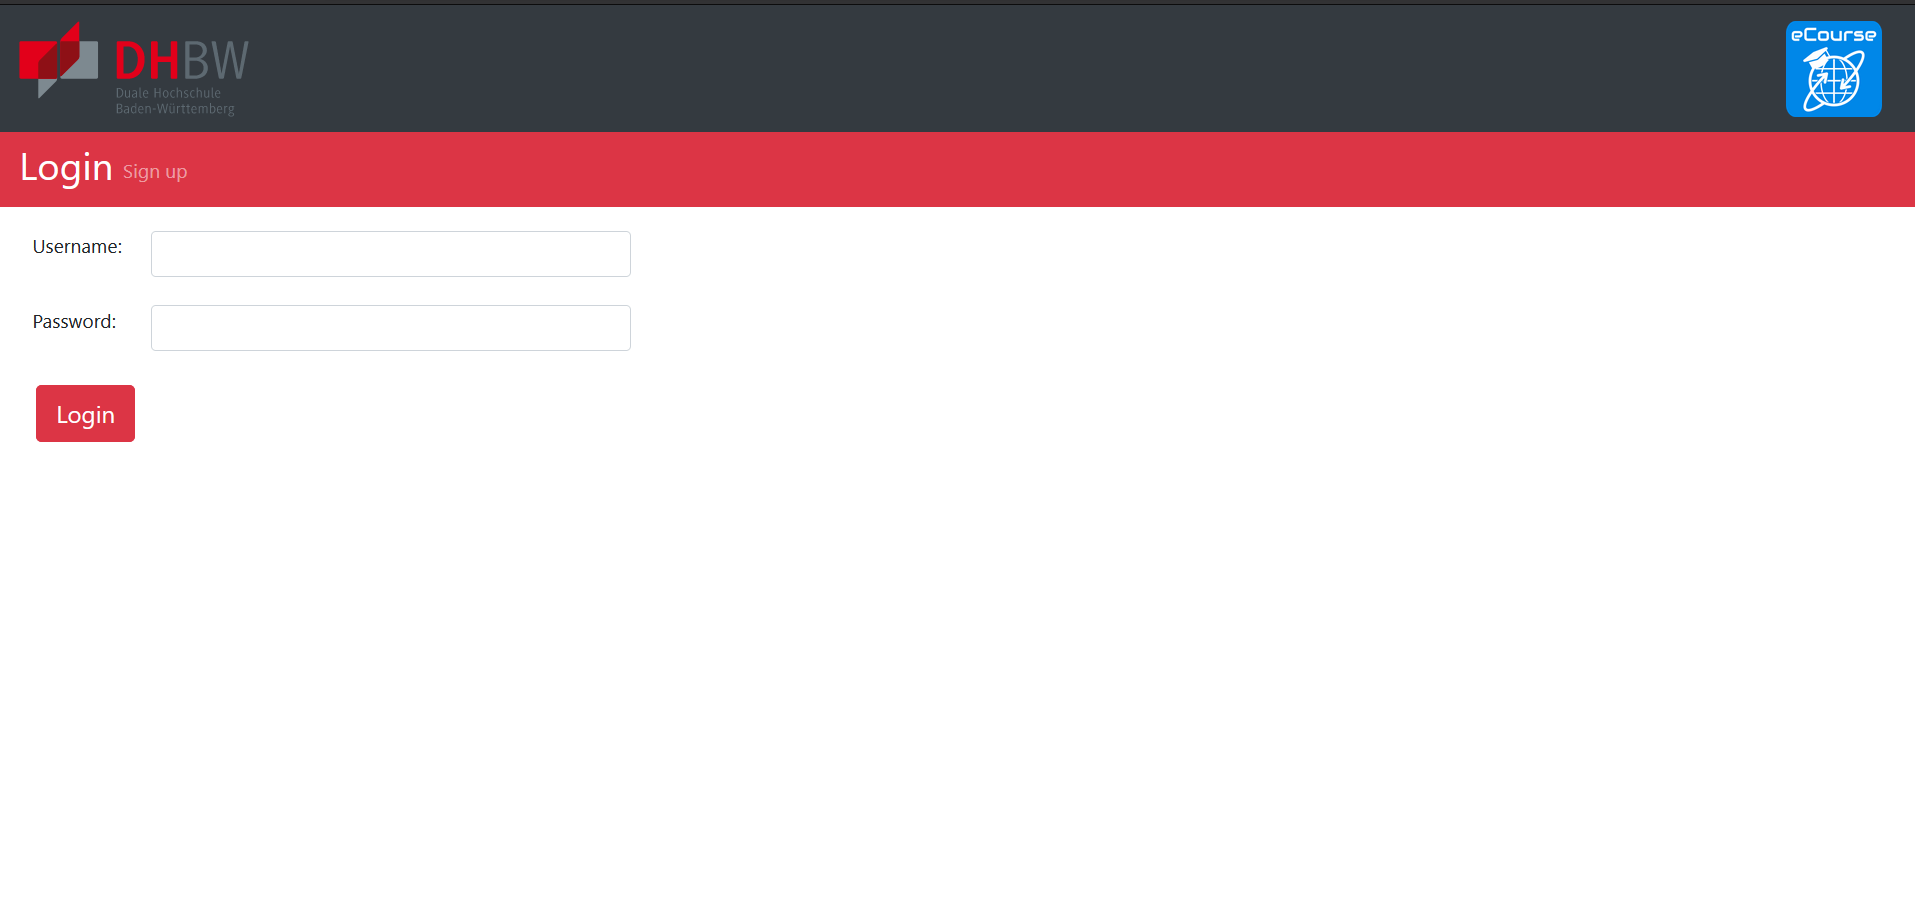
\includegraphics[height=.5\textwidth]{login_page.png}
\caption{Login in die Anwendung eCourse}
\label{fib:Log}
\end{figure}

\textbf{Logout}\\
Möchte der Nutzer seinen Besuch der Anwendung beenden und sich ausloggen, kann er dies mit einem Klick auf die Schaltfläche \glqq sign-out\grqq\: tun. Nach dem erfolgreichen Logout wird der Nutzer wieder auf die Startseite zurück geleitet.
\textcolor{magenta}{hier random bild wo man den logout sieht}